\documentclass[11pt]{article}
% -*-coding: iso-latin-1  -*-
\usepackage{graphicx}
\usepackage{url}
\usepackage{hyperref}
\usepackage{wrapfig}

\usepackage{listings}
\lstset{language=tex}

\usepackage[spanish, english]{babel}
\usepackage[utf8]{inputenc}

%This is for removing coloured boxes around the links and internal references. I don't like those boxes%
\hypersetup{
    colorlinks=false,
    pdfborder={0 0 0},
}


\title{\textbf{\underline{The Technologies}}}
\author{
        Jose Alberto Navas Guerrero (Janague)\\
                Case Studies II\\
       Master's Official Software Libre\\
       Professor: Gregorio Robles\\
	Universidad Rey Juan Carlos\\
        Spain
}

\begin{document}
\maketitle

\begin{abstract}
 This report is a part of an horizontal report about different topic of same projects and in particular this report is about \textbf{the technologies} in these projects: FreeBSD, SilverStripe, Camino, Linux Kernel, Mercurial, Debian, and EdgeBSD. The talks in this subject will show the projects vertically, i.e., they will contain information regarding the history, the goals, the members, the licenses, the related industry, the technologies, the governance, etc of the project. 
\end{abstract}


\begin{center}
\textsc CC BY-SA 3.0\\[0.2cm]

\includegraphics[scale=0.5]{img/by-sa} \\ % Include license
{\small http://creativecommons.org/licenses/by-sa/3.0}\\

\end{center}
\newpage

\tableofcontents

% \listoffigures

\newpage

\section{Introduction}

This report analyzes the used technologies in talks about different free software projects. In general, these talks are not too much technical and they are more oriented to another topics about the communities, like how they create a social process for writing software, and so on.

In every section there is a introduction about project of the talk and technical information about the speaker. And finally, additional information about technologies treated in the presentation.  

%------------------------------------------------------------------------------
% 1. How the FreeBSD Project Works
\section{How the FreeBSD Project Works}

\subsection{Introduction}
\textbf{FreeBSD} is an operating system for a variety of platforms which focuses on features, speed, and stability. It is derived from BSD, the version of UNIX® developed at the University of California, Berkeley. It is developed and maintained by a large community. 

About speaker of this talk, \textbf{\emph{Robert Nicholas Maxwell Watson}} is a FreeBSD developer and has PhD in \emph{computer security}, and founder of the TrustedBSD Project. He is currently employed as a University Lecturer in \emph{Systems, Security, and Architecture }in the Security Research Group at the University of Cambridge Computer Laboratory.

\subsection{Technology}
The talk is about the process of writing open source in a large open source project. And the speaker is interested the following technological topic in operating system security, high performance network and multiprocessing. Watson starts with an introduction to FreeBSD, what the FreeBSD is, what the FreeBSD project is and how it works, who the committers are, the development process and release.

The main objective of the \textbf{FreeBSD} project is the creation of an operating system that can be used without any type of obligations or ties, but that has all the advantages of \emph{code availability} and is \emph{carefully processed }to guarantee the \emph{quality} of the product. Therefore, there are other types of free operating systems, apart from the popular GNU/Linux. The FreeBSD Project had its genesis in the early part of 1993.  

FreeBSD consists of all the components needed for a complete operating system: Multi-processing and multi-threaded kernel, multi-protocol network stack, compiler (UNIX, POSIX, BSD programming interfaces), include files, libraries, user-land, utilities (17.300 third partly software ports, easy portability is an important aspect in the project), and \emph{extensive documentation} (the community is focusing on documentation). 

FreeBSD is intensively used in ISP and as appliance/product/embedded OS foundation. You cannot use the Internet without using FreeBSD.

The good technologies in FreeBSD is not the reason for the success of the project, the reason is that it has a social process for writing software for an active community. 

The Build System and Release System for entire source code for FreeBSD is stored in a \emph{CVS repository}, and the logs, and individual changes for each file can be traced back to 1994. Revision control and revision control is central of development process in this extensive community. And for communication the project is mainly used mailing lists and user groups around the world, and events like conferences and developer summits.

FreeBSD developers maintain at least two branches of simultaneous development. The -CURRENT branch always represents FreeBSD development. A -STABLE branch of FreeBSD is created for each major version number, from which -RELEASE are cut about once every 4–6 months. 

FreeBSD development cycle is based on 18-24 month major ``dot zero'' releases (6.0,7.0. ...) and 4-6 month minor ``dot'' releases (5.5,6.1,6.2, ...). At present, the stable release is 10.0.

Release FreeBSD 7.0 offers many features in multiprocessing: 16+ core scalability, ULE2 scheduler, new threading library and scalable jemalloc; in file systems: Sun's ZFS file system, GJournal for UFS; in networking: Direct dispatch, zero-copy BPF, 10 Gbps optimization, SCTP; superpages, and much more.

Most project activity is in CVS (primary revision control system) and actually four repositories. At that moment, the community is found out technical limitations, there were from 300 to 400 active developers. Four or five years before 2007, they had introduced Perforce, which  is a commercial, proprietary revision control system developed by Perforce Software, Inc. This repository is the secondary revision control system with better features managing many branches.

The future of revision control is difficult to know, since the cost of migration is very high, interrupt development, retain developers, and high risk. In June 2008, development of the base system moved to a different version control system, and in May 2012, the FreeBSD Documentation Project moved from CVS to Subversion. 

FreeBSD currently uses GNATS for its bugtracking system. Some FreeBSD developers think that it could do better. At present, they carry on using GNATS.

The FreeBSD Ports collection is a package management system, providing an easy and consistent way of installing software packages. 

Finally, the FreeBSD project is based on the philosophy of BSD licenses, therefore, the user has the liberty to do whatever they like with the software. Therefore, for this broad freedom there are many technological companies using this operating system for the base of its products. Projects that consume FreeBSD but produce something new and different:FreeSBIE, pfSense, PC-BSD, Darwin, DesktopBSD, DragonflyBSD, FreeNAS,...

\subsection{Additional information}
In this section we include some additional information about FreeBSD Technologies.

In FreeBSD, its \emph{advanced networking}, \emph{security} and \emph{storage} features have made FreeBSD the platform of choice for many of the busiest web sites and most pervasive embedded networking and storage devices. FreeBSD's focus on \emph{performance}, \emph{networking}, and \emph{storage} combines with ease of system administration and comprehensive documentation to realize the full potential of any computer.

FreeBSD includes a number of other great features:

    \textbf{Firewalls}: The base system includes IPFW and IPFilter, as well as a modified version of the popular pf with improved SMP performance. IPFW also includes the dummynet feature, allowing network administrators to simulate adverse network conditions, including latency, jitter, packet loss and limited bandwidth.
    
    \textbf{Jails} are a light-weight alternative to virtualization. Allowing processes to be restricted to a namespace with access only to the file systems and network addresses assigned to that namespace. Jails are also Hierarchical, allowing jails-within-jails.  
    
    \textbf{Linux emulation }provides a system call translation layer that allows unmodified Linux binaries to be run on FreeBSD systems. 
    
    \textbf{DTrace} provides a comprehensive framework for tracing and troubleshooting kernel and application performance issues while under live load.
    
    \textbf{The Ports Collection }is a set of more than 24,000 third party applications that can be easily installed and run on FreeBSD. The ports architecture also allows for easy customization of the compile time options of many of the applications.
    
    \textbf{Network Virtualization}: A container (``vimage'') has been implemented, extending the FreeBSD kernel to maintain multiple independent instances of networking state. Vimage facilities can be used independently to create fully virtualized network topologies, and jailcan directly take advantage of a fully virtualized network stack.

About FreeBSD's \textbf{Internetworking}
\begin{itemize}
	\item FreeBSD was designed for the Internet
	\item FreeBSD supports all standard TCP/IP protocols.	
	\item FreeBSD's networking is stable and fast.
	\item High performance and security.
\end{itemize}


\newpage


%------------------------------------------------------------------------------
% 2. How Open Source Projects Survive Poisonous People
\section{How Open Source Projects Survive Poisonous People}

\subsection{Introduction}
This talk is orientated to community management and conflict resolution, and there are really \emph{few technological aspects} in this talk. In every project runs into people who are selfish, uncooperative, and disrespectful. These people can silently poison the atmosphere of a happy developer community. Come learn how to identify these people and peacefully defuse them before they derail your project.

About speakers of this talk, \textbf{\emph{Ben Collins-Sussman}} is one of the founding developers of the \emph{Subversion version control system}, co-authored O'Reilly's ``Version Control with Subversion'' book as well as ``Team Geek''. Ben co-founded Google's engineering office in Chicago, ported Subversion to Google's Bigtable platform, led engineering teams for both Google Code and Google Affiliate Network, and now manages engineers working on the DFP advertising platform. And \textbf{\emph{Brian Fitzpatrick} }started Google's Chicago engineering office in 2005, and currently leads Google's Transparency Engineering team, which uses data to help protect free expression and free speech on the web. He also founded and leads Google's Data Liberation Front, a team that systematically works to make it easy for users to move their data both to and from Google (e.g. via Google Takeout). He serves as both thought leader and internal advisor for Google's \emph{open data }efforts and has previously led the Google Code and The Google Affiliate Network teams. 
\subsection{Technology}
In the O'Reilly's book ``Producing open source software'' you can find technical details and human aspects of free software development.

Some ideas build a strong community based on politeness, respect, trust, and humility.

Best practices, first having a concrete direction, for example, subversion goals is ``To create a compelling replacement for CVS`` (maybe they had to choose a objective more concrete and ambitious), it should be something that community should focus on it.

Besides, they talked about how to use mailing list etiquette, documentation, VCS, bug tracking system, release management, governance.

\subsection{Additional information}
Most free software projects offer at least a minimum, standard set of tools for managing information:
\begin{itemize}
	\item Web site of the project. With documentation, such as developer guide, user manual.
	\item Mailing lists / Message forums
	\item Version control system
	\item Bug tracking system
	\item Real-time chat
	\item Release and packages management system
\end{itemize}

\newpage


%------------------------------------------------------------------------------
% 3. SilverStripe CMS
\section{SilverStripe CMS}

\subsection{Introduction}
SilverStripe is a free software Content Management System (CMS) and Framework for creating and maintaining websites and web applications. It provides an out of the box web-based administration panel that enables users to make modifications to parts of the website, which includes a WYSIWYG website editor. The core of the software is SilverStripe Framework, a \emph{PHP Web application framework}.

About speakers of this talk, the main speaker was \emph{\textbf{Sigurd Magnusson}}, who is one of SilverStripe’s three co-founders. He works full-time in the business and focuses on \emph{sales and marketing}.  Sigurd's strong technical ability and excellent people skills add valuable depth to SilverStripe. While now less involved with \emph{programming}, his interest and experience with the technologies that form the Internet make him extremely useful in identifying how technology can be used to push boundaries and solve human challenges. Sigurd is an evangelist for the principles and technology of the web, and is an avid supporter of open source, open data, and the web as a modern software platform.

In technical questions was speaking\emph{ \textbf{Sam Minnée}}, CEO and co-founder of SilverStripe keeps the company focused on its mission to reshape business through the web. Sam has a \emph{BA in Computing} and Philosophy from Victoria University.

\subsection{Technology}
Firstly, Sigurd introduces New Zealand data, in particular, he talks about free software projects with New Zealand contributors, like Jade, Aftermail, Xero, PGP, PlanHQ, and Catalyst. And example of usage of free software like democratic process, which is implemented with Perl/Mason and Postgres. 

Again the O'Reilly's book ``Producing open source software'' is seen as the Bible of free software development.

Their experience in Google summer of code was the following developments:
\begin{itemize}
  \item Mashups: Gallery of pictures, forum...
  \item Internationalisation: Is interesting, label you need a system to manager.
  \item Usability: A lot of things to incorporation, draw and drop files, buttons
  \item Google Adwords and Sitemaps: integrate very nice in the system.
  \item Google Maps: Geolocalitation
  \item Postgres, MS SQL support (via PDO)
  \item Image Manipulation, in relation with usability.
  \item Reporting: Uses canvas (HTML/CSS/JavaScript) and not Flash/Image files. Small piece of code.
  \item Safari support, solving problem about Javascript, XML and CSS.
  \item openID: Providers or directories.
\end{itemize}

\subsection{Additional information}
SilverStripe separates the roles of content authors (who get a rich (AJAX) web-based user interface that omits technical jargon) and website designers/developers (who write code: HTML, CSS, JavaScript, and PHP).

The core of SilverStripe is named SilverStripe Framework. SilverStripe Framework is an object-oriented PHP5 web application framework. It is based on a Model-view-controller (MVC) architecture, a popular approach for building web-based applications. SilverStripe Framework reduces the overhead associated with common programming tasks, and enables developers to write code in a logical and structured manner.

SilverStripe generates markup using a custom template language based on W3C HTML5 that offers simple placeholders and conditional logic. SilverStripe is extensible through modules, widgets, themes, code customization, and ModelAdmin.

SilverStripe is released under the terms of the BSD License. 

\textbf{PHP} (recursive acronym for PHP: Hypertext Preprocessor) is a widely-used open source general-purpose scripting language that is especially suited for web development and can be embedded into HTML. 

The \textbf{i18n class }(short for ``internationalization'') in SilverStripe enables you to display templates and PHP code in different languages based on your global settings and the preferences of your website users. This process is also known as l10n (short for ``localization'').

The \textbf{PHP Data Objects (PDO)} extension defines a lightweight, consistent interface for accessing databases in PHP. Each database driver that implements the PDO interface can expose database-specific features as regular extension functions. PDO provides a data-access abstraction layer, which means that, regardless of which database you're using, you use the same functions to issue queries and fetch data. PDO does not provide a database abstraction; it doesn't rewrite SQL or emulate missing features. You should use a full-blown abstraction layer if you need that facility. 

\textbf{OpenID} is an open standard that allows users to be authenticated by certain co-operating sites (known as Relying Parties or RP) using a third party service, eliminating the need for webmasters to provide their own ad hoc systems and allowing users to consolidate their digital identities.

\textbf{Ruby on Rails,} often simply Rails, is an open source web application framework which runs via the Ruby programming language. It is a full-stack framework: it allows creating pages and applications that gather information from the web server, talk to or query the database, and render templates out of the box. As a result, Rails features a routing system that is independent of the web server. Ruby on Rails emphasizes the use of well-known software engineering patterns and principles, such as active record pattern, convention over configuration (CoC), don't repeat yourself (DRY), and model–view–controller (MVC).

\newpage


%------------------------------------------------------------------------------
% 4. Camino
\section{Camino}

\subsection{Introduction}
Camino was a free, open source, \emph{GUI-based Web browser} based on \emph{Mozilla's Gecko }layout engine and specifically designed for the OS X operating system. In place of an XUL-based user interface used by most Mozilla-based applications, Camino used Mac-native Cocoa APIs. On May 30, 2013, the Camino Project announced that the browser is no longer being developed.

About speaker of this talk, \textbf{\emph{Mike ``Pink'' Pinkerton}} is an American \emph{Software Engineer} who is known for his work on the Mozilla browsers. He lectures on \emph{Development of Open Source Software} at George Washington University. Pinkerton studied at University of California, San Diego where he graduated with a B.S. in \emph{Computer Science}, then at Georgia Institute of Technology where he graduated with a Master's Degree in Computer Science. Pinkerton started working at Netscape Communications in June 1997 where he worked on the Netscape Navigator and then Mozilla browsers, and worked to opening source code for Netscape. While at Netscape he started development of the Camino (then Chimera) web browser with Dave Hyatt.  Mike Pinkerton had been the technical lead of the Camino project since Dave Hyatt moved to the Safari team at Apple Inc. in mid-2002.

\subsection{Technology}
Mike Pinkerton talk about the past, present, and future of Camino project, and lessons learned from Netscape development, open source in Mozilla, and Camino development.

In 1998 Microsoft Internet Explorer was for free and the market share was growing up, thus the business model of selling Netscape product was in risk. They realized that they had to change the rules (Maybe there was not really nothing else to do), and they did. Netscape make the important and original decision to open source of all product and the all of the technologies involved.

Source331 project was a Netscape project to all-out effort to have the source code of its suite Netscape communicator out by March(3) 31, 1998. Outstanding fact for free software history.

Netscape had  a cross-platform history of its products, and in that moment there were not resource for maintained all the developers team, only for the MS Windows. But the designers had expert knowledge of web standards (HTML, DOM, javascript, CSS, XML) and programmers of the community the capacity, and something so magic happened, the project worked, and release building alone for the community, without company paid for that.

But there were problems, one of them the need to release a version, thus in 2000 Netscape 6 was release, and it was very bad. Until version 6.2 the product was not stable. Another problem was that Windows oriented design constrained portability. And at that moment an opportunity appeared with Apple to create a new browser using Cocoa browser and gecko engine for Mac. 

But when it was finished with high quality, a manager of the company decided that two browsers were enough, Netscape 7 and IE. Then it was a really disappointment for that, and he decided to create a free software project, Camino.

Lesson learned were

Openness. User should be centric of the project, and users and developer should take part of the community, and the project should provide system for that: User forum, Q\&A, website user centric.

Weak ownership:	Testers are the most valuable resource, and usually are users, and weak ownership attracts users to collaboration. The project should provide testing and bugs tracking system, although browser projects are difficult of testing, since there are many range of contents, different languages, proxies, security, and so on.
	
The future of Camino at that time was Leopard-only to take full advantage of OS; 	Webkit (layout engine) is faster rendering the web, and it has important advantage of Gecko, Gecko is very complicated and unapproachable system,  and so its learning curve is tremendous; and continue association with Mozilla Foundation.
	
\subsection{Additional information}

\textbf{WebKit} is a layout engine software designed to allow web browsers to render HTML (is not only on web pages). Become a FLOSS project in 2005 when Apple released the code. Is used in Mac OS X system framework with Safari, Dashboard, Mail, and many other OS X applications. Also you can find WebKit in Nintendo 3Ds, Kindle and Android. This project started as a branch of the KHTML and KJS libraries from KDE. It is a community made up by companies: Apple, Nokia, Google, RIM, Igalia, Samsung.

After a decade long run, Camino is no longer being developed, and we encourage all users to upgrade to a more modern browser. Camino is increasingly lagging behind the fast pace of changes on the web, and more importantly it is not receiving security updates, making it increasingly unsafe to use.

\newpage


%------------------------------------------------------------------------------
% 5. Greg Kroah Hartman on the Linux Kernel
\section{Greg Kroah Hartman on the Linux Kernel}

\subsection{Introduction}
The talk is about who is developing the Linux kernel, how they are doing it, and why you should care. Free software development violates almost all known \emph{management} theories. Talking about processes of development kernel.

About speaker of this talk, \textbf{\emph{Greg Kroah-Hartman}} has been building the \emph{Linux kernel} since 1996 and started writing Linux kernel drivers in 1999. He is currently the maintainer of the \emph{USB, PCI, driver core and sysfs subsystems} in the kernel source tree and is also one half of the -stable kernel release team. He created the udev program and maintains the Linux hotplug userspace project. He is a Gentoo Linux developer as well as the co-author of the third edition of the ``Linux Device Drivers'' book and a contributing editor to Linux Journal. He also created and maintains the Linux Device Driver Kit. He currently works for SuSE Labs/Novell, doing various Linux kernel related tasks. 
\subsection{Technology}
The Linux kernel is a stunning dynamic large project, at that moment it had the following rate of changes per day in 2007
\begin{itemize}
	\item 4,300 lines added
	\item 1,800 lines removed
	\item 1,500 lines modified
\end{itemize}
The kernel source code is about 9 million lines of code, the core of kernel is 5\%, drivers around 50\%. And the rate changes is proportional, and uniform respect core or drivers, thus it is flat in rate of changes.

At that moment, 3.69 changes per hour 24x365, in 2.6 release 2.5 changes per hour.

\hfill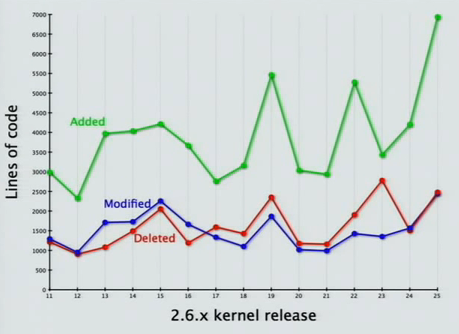
\includegraphics[scale=0.8]{img/26kernelChanges}\hspace*{\fill}

and the trend is going up.

\hfill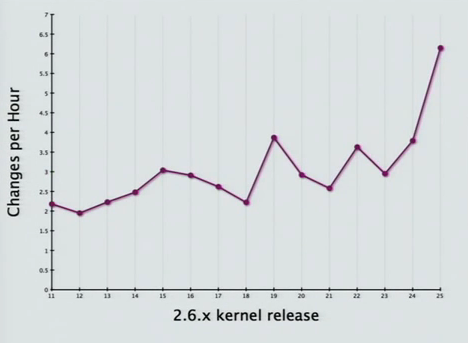
\includegraphics[scale=0.8]{img/changePerHour}\hspace*{\fill}

With this data, is it stable kernel? How do they do this? 

First, the development process is open manner, chaotic manner, and fast manner. At that moment, there were more than 2.000 developers, 600 maintainers (as curiosity the graph is 40 feet long and 4 feet tall). Each level consolidate its subsystem. 10\% lines code more per year
2399 developers, that's amazing, half of these contributors only contributed one patch. Its a exponential curve. The top 200 people - 80\%
commits.

\hfill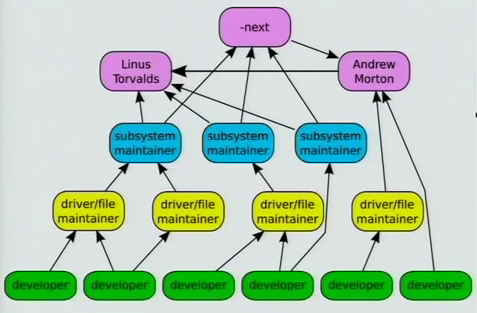
\includegraphics[scale=0.7]{img/organizationKernel}\hspace*{\fill}

The Build System and Release System for entire source code for Linux is stored in a \emph{GIT repository}, there is no stable and unstable development trees. They changed the model to release each 2 3/4 months, like clockwork. The security (x.x.x.[1,2,3,...]) bug only is update in a new branches, even in hours soon as possible.  

The Testing System,	they cannot have standard unit test because there is no good way to test it, no automated system, the community of developers and user testing new releases. 	Performance test is also hard. Track regressions using the last bugs.

Quantity, Top 10 developers
\begin{itemize}
	\item Adrian Bunk - janitorial patches
	\item Al Viro - BFS
	\item Thomas Gleixner - i386 X86
	\item David S. Miller - Networking Core
	\item Bart Zolnierkiewicz - IDE
	\item Paul Mundt - SH
	\item Ralf Baechle - MIPS
	\item Ingo Molnar - NetFilter
	\item Patrick McHardy -NetFilter
	\item Tejun Heo - Lab ATA, disk driver
\end{itemize}	

And video and wifi are very active areas.

Who funding this work, the first position with 18.5\% Amateurs.

A particular case, Google, 27 its employees contributed to the kernel in 2007-2008
\begin{itemize}
	\item Andrew Morton - Core Kernel
	\item David Rientjes - NM and out of memory stuff
	\item Paul Menege - CPU scheduling
	\item Ken Chen - Core Kernel, TLB
	\item Matt LaPlante - Spelling fixes to the kernel
\end{itemize}

The user interface should be stable and stay the same. Move slowly, like ``UNIX'' or Windows model, but the API inside the kernel is changed all the time. The stable model of kernel, for instance security appliances, is only the 20\% of the market, the rest you usually need to change HW then you need to change kernel.

What are coming.
KVM (AMD and intel) makes Linux be the hypervisor. The way it has a kernel, XEN model there are their own scheduling, their own memory management or their power management. The amazing thing is that is real time. You can now real time schedule these guest operating systems, so people can measure network latency and processes latency. Guest operating systems run as a process. Xen cannot do that.

In conclusion, Linux is not a intelligent design, it is an evolution design. For that, the Linux project has achieved a development rate of change amazing and efficient development model.

\subsection{Additional information}
At present, the 3.10 Linux Kernel Development Rate is completely stunning. Every year you could think that developer team cannot go faster, and every year you are wrong.

\hfill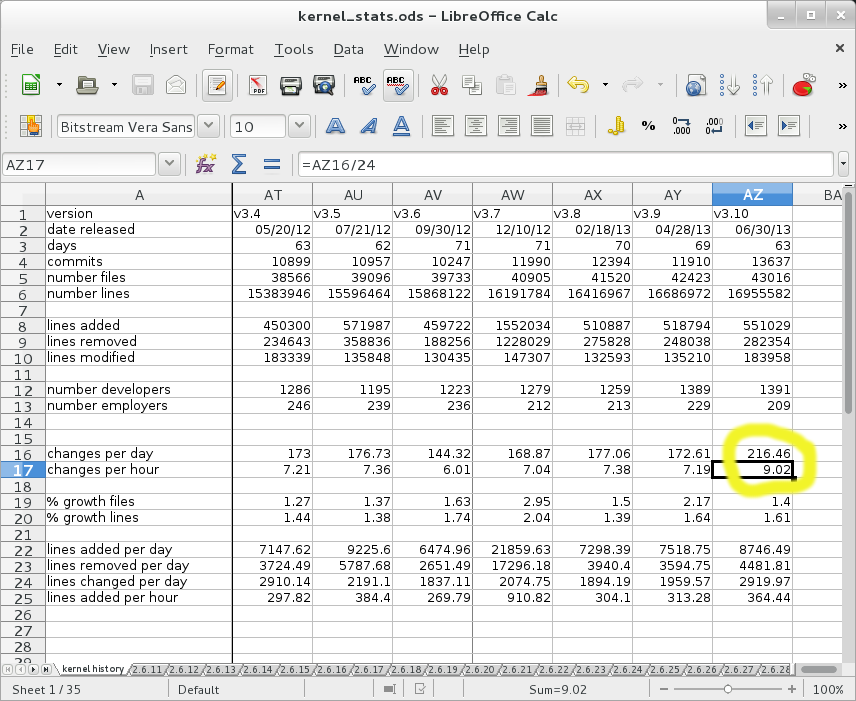
\includegraphics[scale=0.4]{img/kernel310rate}\hspace*{\fill}

\newpage

%------------------------------------------------------------------------------
% 6. Mercurial Project
\section{Mercurial Project}

\subsection{Introduction}
Mercurial is a free \emph{distributed revision control system}. It focuses on conceptual simplicity, robustness, and high performance. Well-known open source projects that use Mercurial include OpenSolaris, Xen, and One Laptop Per Child. This talk presents some of the advantages of using Mercurial to manage large, fast-moving projects.

About speaker of this talk, \textbf{\emph{Bryan O'Sullivan}} is an Irish writer and \emph{developer} who works with \emph{distributed systems}, \emph{open source software}, and \emph{programming languages}. He wrote the award-winning O'Reilly title Real World \emph{Haskell}. He has made significant contributions to the popular Mercurial revision control system, and to a number of other open source projects. He lives in San Francisco with his family. 

\subsection{Technology}
Mercurial is a free distributed revision control system, which does tasks very fast. It is implemented 95\% in python and 5\% of core in C for speed programming languages. And it is implemented in 12.000 lines of code.

Projects:
\begin{itemize}
	\item Linux: video4linux, ALSA, e2fsprogs, ...
	\item System software: Xen, OpenSolaris, Conary, FreeBSD ports, ...
	\item Other exciting projects: One Laptop Per Child, Moin Moin, microformats, physics textbooks, ...
\end{itemize}

There are three important concepts:
\begin{itemize}
	\item Repository - It contains the history of a project, and it is implemented using a directory. A repository can clone very easy since it is a directory. Thus, every developer works with his own repository.
	\item Working directory - It is a copy of a part of a project. All files are modificable, and a modification will be saved when it is committed.
	\item Changeset - A snapshot of the project at a point in time, with information about committer, readable description of the change, list of changed files, and parent changeset.
\end{itemize}

Mercurial will scale to large projects better than other revision control system written in C, because of the underlying instructions that they use and implementation techniques.

Mercurial has got as many as central repositories needed, no only one like traditional SCM. There is not central server and so you can work in local without to be connected with central server, thus every developer has a full backup of the project and he is fully productive even without network connection.

In conclusion, Mercurial is easy to use, robustness, and really fast performance. And written in Python, at least initially no high performance language, but the used techniques in the implementation give Mercurial this high performance. 

\subsection{Additional information}
\subsubsection* {Interoperability Tools}
Mercurial has the convert extension, which does a great job of converting repositories from some other system to mercurial. It's clean, consistent, and fast.
\subsubsection*{ Branch Management}

In Mercurial there are two types of branches you might see as a user: named branches and repository clones. Cloning a repository is how you branch in darcs and is a really simple concept. When you want to do something different, you just clone your repo somewhere else and start working. Named branches allow you to have a workflow where you can switch back and forth between branches in the same working directory. However, named branches are flawed.

In Mercurial, every changeset belongs to a named branch. That is, the branch name is stored in the changeset. The flaw is that it's quite easy to have more than one branch with the same name, and it's difficult to tell when this has happened. This can cause confusion in a team where one is left wondering what changes, exactly, have made it into the stable branch when multiple people have reopened and merged the branch on different timelines.

Also, because the branch name is in the changeset, the branch lives forever. The only short-term branches are clone branches. That just doesn't encourage quick experiments.



\newpage

%------------------------------------------------------------------------------
% 7. Stefano Zacchiroli on Debian: 20 Years and counting
\section{Stefano Zacchiroli on Debian: 20 Years and counting}

\subsection{Introduction}
Debian is one of the eldest Free and Open Source Software (FOSS) distribution in existence. The project has been founded in 1993 to further Free Software distribution and is still doing so in an purely community-driven way. The Debian Project and distribution are both made by volunteers who employ a dual ``do-ocratic'' (a form of meritocracy based on the outcome of individual work) and democratic model to make decisions and drive Debian toward its goals. The uniqueness of Debian is manifest in its Free Software values, independence from commercial interests, and in its importance as the basis of a huge ecosystem of several hundreds derived FOSS distributions, which includes today's most popular ones. 

About speaker of this talk, \emph{\textbf{Stefano Zacchiroli}} is Associate Professor of \emph{Computer Science} at University Paris Diderot. His research interests \emph{span formal methods} and their applications to improve \emph{software quality} and user experience in the context of \emph{Free Software distributions}. He has been involved in the Debian Project since 2001, taking care of many tasks from package maintenance to distribution-wide Quality Assurance. He has been leading the Debian Project since April 2010.

\subsection{Technology}
In this talk they present the Debian Project and distribution, discuss its unique traits, as well explain how to join the Project and contribute to it.

The process of install some package some years ago: Download tar.gz, ./configure, foreach, make, and make install.

At present, there are project that upstream software and distribution editors create package in a package repository, which users can use using package managers, like application stores of other platform.

In the origin of Debian project, 20 year ago, Ian A Murdock make a GNU/Linux competitive with commercial OS, easy to install, and built \emph{collaboratively} by software experts, also in distribution.

At present, the community offers a Operation System, called Debian stable, with a binary distribution, completely free, released every 24 months, a dozen architectures, and archive-wide security support for all packages (3-3.5 years), good documentation.

\underline{\emph{Debian 6.0 ``Squeeze''}}
\begin{itemize}
	\item Completely Free Linux kernel, firmware included.
	\item New kernel, kFreeBSD.
	\item Most popular GNU/Linux on the Web (32.7%)
	\item New services: Snapshot, backports, stable-updates, screenshots, and ask.
\end{itemize}

\underline{\emph{Debian 7.0  ``Wheezy''}}
\begin{itemize}
	\item Multiarch: 	Proper technical way of sharing packages across archs, like 32 bits and 64 bits packages in the same machine. Cross-compilation.
	\item Private cloud deployment:  OpenStack, Xen/XCP, OpenNebula
	\item Public cloud support: EC2, Azure, ..
	\item New archs: armhf, s390x
	\item Desktop: Gnome 3.4, KDE, Plasma 4.8, XFCE.
\end{itemize}

\emph{Communication channel}: Mailing lists, IRC, a few Web services growing, like social @debian, !debian on identi.ca.

Development processes

\hfill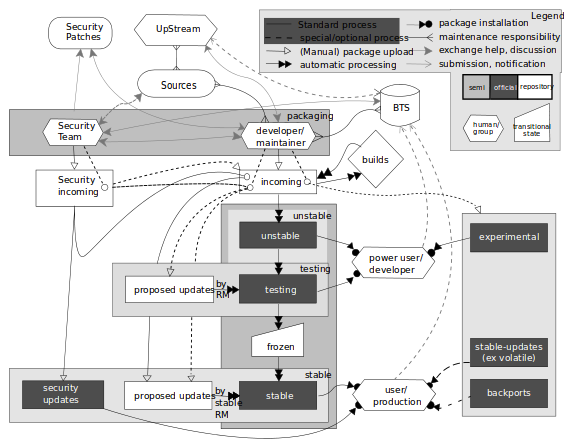
\includegraphics[scale=0.6]{img/DebianDevelopmentProcess}\hspace*{\fill}
	
	\emph{Debian's special \#1}: Package quality
		There is a culture of technical excellence, to that effect, there are a policy of package design; a package testing suite: lintian, piuparts, archive rebuilds (FTBFS),...; the package maintainers are software experts; and all packages are treated in the same level of requirements.
	Debian is released when it is ready.

	\emph{Debian's special \#2}: Freedom
	Software of the distribution is free software, included firmware; but in its infrastructure also is used free software, in web services for users and infrastructure for developers. And so, freedom makes a condition of what techniques uses in Debian.

	\emph{Debian's special \#3}: Independence

	\emph{Debian's special \#4}: Decision making
	\begin{itemize}
			\item \emph{do-ocracy}: An individual Developer may make any technical decision with regard to their own work.
			\item \emph{democracy}: Some technical decision in the project is made by one o more developers.
	\end{itemize}

At that moment, there were around 140 active derivative from Debian.
		
Analysis of particular distribution: Ubuntu
\begin{itemize}
	\item 78\% Debian
	\item 12\% patches of Debian
	\item 10\% no Debian packages
\end{itemize}
	
In the past ten years Distribution Model was quite simple, only one distribution, and bug reports and parches only applied to a single distribution. At present, the ecosystem is much more complex, with many users and developers using different distribution, where users report bug of particular distribution, it flows to the Debian upstream if it is apply. This model has got some advantages more potential contributors, more bugs, more patches installed and so more tests. But the model should be sustainable.

\subsection{Additional information}
\textbf{Debian GNU/kFreeBSD} is a general purpose operating system, an official Debian GNU distribution using the kernel of FreeBSD instead of the Linux kernel. About ninety percent of the Debian software archive is available for Debian GNU/kFreeBSD.

\textbf{Xen Cloud Platform }(XCP) is the open source version of XenServer, which is a Citrix commercial product. It's of course based on the Xen hypervisor. XCP is written mainly in the OCaml language, with some parts also written in Python and C. It is a very mature product, which works easily, and is fairly easy to install. 

\newpage

%------------------------------------------------------------------------------
% 8. The EdgeBSD Project
\section{The EdgeBSD Project}

\subsection{Introduction}
\textbf{EdgeBSD} is a new member of the family of \emph{BSD-based Operating Systems}, starting development with the current NetBSD codebase with \emph{Git for Source Code Management}. Package management is based on pkgsrc.

About speaker of this talk, \emph{\textbf{Pierre Pronchery}} is a \emph{Computer Science post-graduate} (BSc, Oxford Brookes) and \emph{engineer} (INSIA). With a broad culture of Operating System internals, software design and network architecture, development or assessment activities: \emph{Source code auditing }(C, UNIX, PHP...), \emph{reverse-engineering} (binaries, firmwares, protocols...), \emph{penetration testing} (host, network...), \emph{porting software} to Linux or BSD (C/C++, Gtk+...), writing \emph{hardware drivers} for Linux or BSD platforms (consumer, server, embedded...). He were working in these projects: DeforaOS, NetBSD, and now EdgeBSD.
\subsection{Technology}

Pierre Pronchere talked about a new family of BSD-based Operating Systems in FOSDEM 2014, which is based on NetBSD and called \textbf{EdgeBSD}, but with a \emph{more open development model} and using git as VCS. He believes the current development model of NetBSD is harmful for its development. In summary, the story of a fork. And in the second part of the speech he shows the configuration of the git repository, and project wiki.

NetBSD has c\emph{lean architecture} and \emph{portable}. With \emph{transparent cross-compilation}. With lots of features ASLR, CGD, Xen, RUMP, ZFS, Dtrace...

There are some potential harms, like NetBSD maintains its own version of GCC, Xorg, Bimd, Postfix,... Therefore, you cannot run NetBSD on 2008 workstation or 2009 laptop with current upstream Xorg package for instance.
	
A comparison between widely used VCSs, CVS and git, whereas CVS is simple and easy to fix, git might be inconsistent and opaque in his opinion. But Git has got lots of features to work in a distributed and decentralized way, work offline with history and branches, branch almost for free, stash and stage and commit and combine, ...

The EdgeBSD is a full copy of NetBSD's sourcecode (src) and packages source(pkgsrc). They had created repositories with NetBSD's original code: netbsd-src, and pkgsrc. And including new features: ASLR (known bugs), SSP (imposes restrictions), secure levels, veriexec, modular kernels, modular Xorg from packages.

In the Open Source development area they want to provide different channel of communication, email,calendar, secure IM, VoIP, conferencing, and so on; and automated checks and procedures.

In the stable release engineering procedure, they want to release a stable version with milestones and continuously, based on NetBSD's stable branch, with extra features, with continuous security and bugfix updates, new packages and easier ways to install (graphically and text-based installers) and deploy in range of devices (like tablets and mobiles).

In the second part of the talk, more practical, Pronchere made the configuration of git repository (netbsd-src, pkgsrc), and set up things like read and write permission users, developers (at present 6 developers). Besides, he shows the project wiki, where you can find information about project organization (roles), and binary repository server for many architectures and packages too.

Every packages have to be signed for installing, and Pronchere shows how to update a packages (pkgin update, pkgin install package). A usual package contains PKG\_HASH file (a bunch of hashes), PKG\_GPG\_SIGNATURE file (pkg\_admin is used for signed packages), and tgz file with the package.

In the following url you can find NetBSD source code in github repository \url{https://github.com/jsonn/src}.

\subsection{Additional information}
For Pronchery, EdgeBSD should be as attractive a platform as possible, and use the advantages of its existing codebase to experiment on being a modern, safe, and portable Operating System. This vision currently includes:
\begin{itemize}
    \item advanced facilities for developers (patch management, build environments...);
    \item re-organization of the base system (Git submodules, packages...);
    \item a graphical installer;
    \item modern package management (signed packages...);
    \item alternatives to Xorg and default desktop environment;
    \item ready-to-flash images for embedded devices;
    \item virtualization of most components with the RUMP anykernel.
\end{itemize}

Finally, most used BSD flavors and its strength
\begin{itemize}
	\item FreeBSD - Maximum performance.
	\item OpenBSD - Maximum security.
	\item NetBSD - Maximum portability.
	\item DragonFly BSD - Emphasis on multiprocessor systems and clustering.
\end{itemize}

\newpage

%------------------------------------------------------------------------------
% 9. Debian Secrets what I wish I knew before joining Debian
\section{Debian Secrets what I wish I knew before joining Debian}

\subsection{Introduction}
Debian is usually advertised as a volunteer project with a subtle mix of democracy and do-ocracy. While this is correct, implementation details are mostly undocumented, and it is often difficult for prospective or relatively new contributors to really understand the inner workings of the project.

This talk will detail some useful lessons, and also some secrets about Debian learned over the years. With the goals of showing the inner working of Debian, and giving some directions to prospective contributors.

About speaker of this talk, \emph{\textbf{Lucas Nussbaum}} is a Debian \emph{developer} and was elected leader of the Debian project in April 2013. He is a \emph{computer science engineer} and \emph{assistant professor} at University of Lorraine, researcher at LORIA laboratory. He has been involved in many areas of Debian over the years, but his main interests are in \emph{Quality Assurance} and \emph{Ruby packaging}. He was also involved in improving collaboration with Ubuntu.

\subsection{Technology}
In Debian, contributors are technological experts in the area of each packages are about. It exists the Culture of technical excellence, you can find really technological discussion in the most high level in the different channels of communication in the project.

There is a Technical Committee to resolve disagreement in design and implementation, but it is only a last resort option and usually take months to resolve it. The Technical Committee is made up by 8 members, and rarely overrules the maintainers, for instance, only one time in 2012 (multiarch/dpkg).

Debian Developers should focus on technical issues, offer solutions (help, patches), no personal issues about the maintainer. It is important to track the development and design of contributors, there is a no-write rule that Not develop anything without informing about how it is going to do that.

For Debian Developers in a team is really important to give feedback is really important, even if it is \emph{empty} positive feedback.

There is a entry barrier as Debian Developer because the documentation is not completed enough, and you usually need help in the first steps, and the best way it is taking part in a team or adopt a orphan package.

Debian project uses a kit tools for packages management, like aggregator PTS (Package Tracking System), DDPO (Developer Package Overview), and UDD (Ultimate Debian Database) 

The general needs of packaging teams are different, some of them working in a few large packages and others in many small packages, some of them use SVN or git, and different tool for management, like  cdbs, dh, parches management, or quilt.  Thus, the development environment is heterogeneous respecting to used technologies in each team. 

snapshot.debian.org is a Debian service with data and graphs about packages management. In the following graphs we can see some examples. 

\underline{Debian co-maintenance evolution}

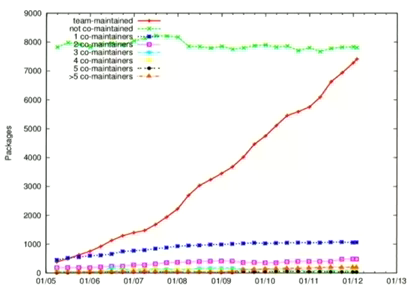
\includegraphics[scale=0.7]{img/comaintenance}

\underline{Debian package formats and patches evolution }

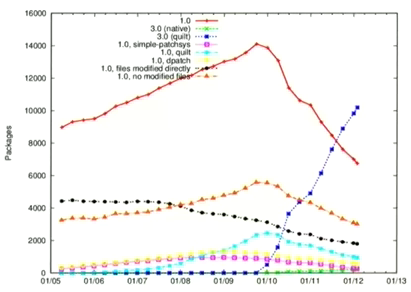
\includegraphics[scale=0.7]{img/package-formats-patches}

At present, the tend is to migrate to new packages format quilt 3.0.

\underline{Debian package helpers}

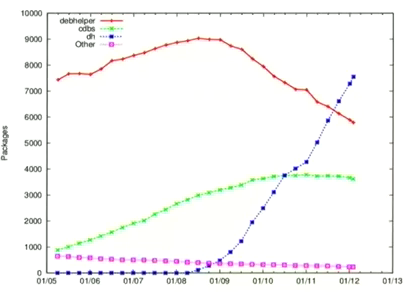
\includegraphics[scale=0.7]{img/packagesHelpers}

dh is introduced in 2008 and at present it is the most popular.

\underline{Debian VCSes}

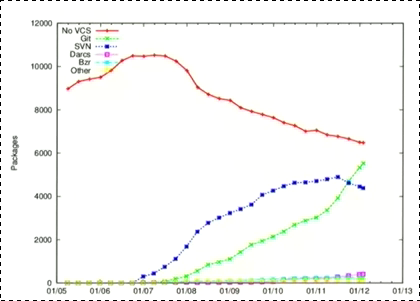
\includegraphics[scale=0.7]{img/VCSes}

Git is now the most popular option for VCS.

Finally, in the following image you can see the general packaging workflow.

\hfill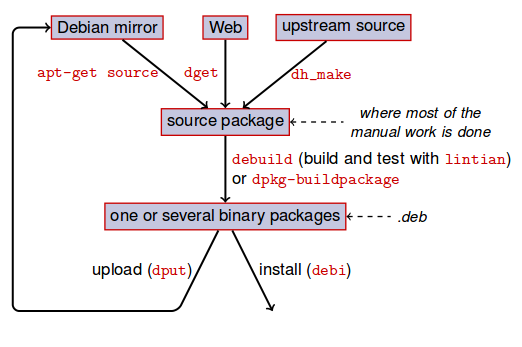
\includegraphics[scale=0.5]{img/generalPackagingWorkflow}\hspace*{\fill}

In conclusion, there are several patterns that you have to take in consideration when you contribute to Debian project. Debian is a vertical and heterogeneous organization in general and technical aspects in particular.

\subsection{Additional information}
A \emph{do-ocracy} is an organizational structure in which individuals choose roles and tasks for themselves and execute them. Responsibilities attach to people who do the work, rather than elected or selected officials.

The \emph{Technical Committee} is established by the Debian Constitution. It is the body which makes the final decision on technical disputes in the Debian project. The decisions can be viewed in the bug tracking system, and there have been few of them, for example, in 2013 only 1, 10 in 2012, 0 in 2011, 1 in 2010, and so on.

The \emph{Package Tracking System(PTS)} lets you follow almost everything related to the life of a package. It's of interest for co-maintainers, advanced users, QA members, ...

The \emph{Debian Developer's Package Overview (DDPO)} is a web application offering a customized overview of all packages of a given maintainer. 

The \emph{Ultimate Debian Database (UDD)} gathers a lot of data about various aspects of Debian in the same SQL database. It allows users to easily access and combine all these data.

The \emph{snapshot archive }is a way back machine that allows access to old packages based on dates and version numbers. It consists of all past and current packages the Debian archive provides. 

\newpage

\bibliographystyle{abbrv}
\bibliography{caseStudiesIIReport}

 \nocite{*}

\end{document}
